\begin{table*}[t]
  \centering
  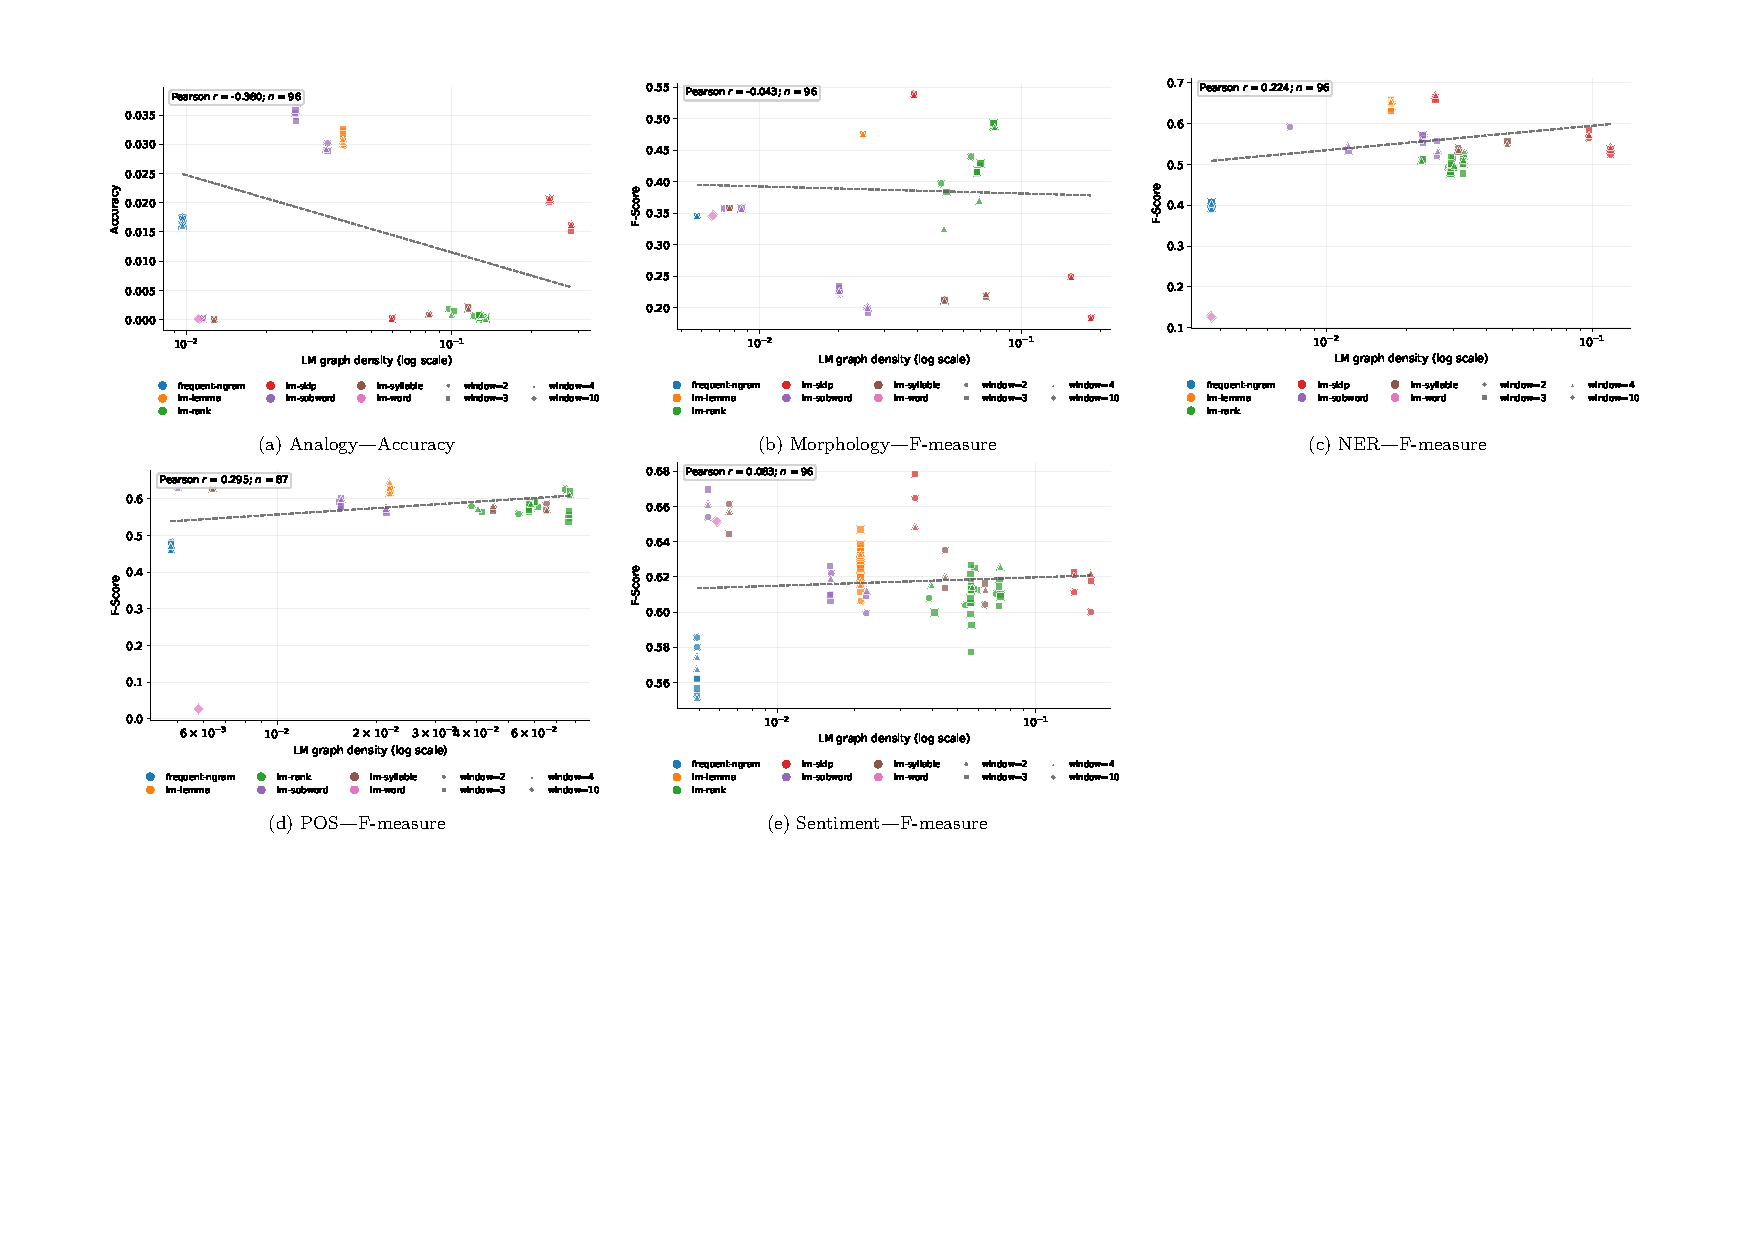
\includegraphics[
    width=\textwidth,
    keepaspectratio
  ]{plots/lm_graph_density_3x2_table.pdf}
  \caption{Relationship between LM graph density and task performance.
  Density is shown on a logarithmic scale. Analogy is evaluated with
  Accuracy, while Morphology, NER, POS, and Sentiment are evaluated with
  F-measure.}
  \label{tab:density}
\end{table*}

\subsection{LM graph density and task performance}

Table~\ref{tab:density} relates the density of the graph induced by each
partitioned corpus to downstream performance. Following the implementation in
\texttt{LMDataset}, graph density is calculated as
$D=2E/[V(V-1)]$, where $E$ is the total weight of the ordered within-sentence
connections between LM partitions and $V$ is the number of distinct
partitions in a deterministic sample of at most 10,000 non-empty sentences.
Thus, denser graphs indicate that the observed partition vocabulary is
connected more frequently within sentences \citep{west2001}. Density is shown
on a logarithmic scale because its empirical range spans more than one order
of magnitude. The task metric follows the rest of the analysis: Accuracy is
used for Analogy, whereas F-measure is used for Morphology, NER, POS, and
Sentiment.

The results do not support a uniform relationship between graph density and
task performance. The descriptive Pearson correlations between log-density
and task score are approximately null for Morphology ($r=-0.043$) and
Sentiment ($r=0.083$). NER ($r=0.224$) and POS ($r=0.295$) show weak positive
associations, whereas Analogy shows a moderate negative association between
log-density and Accuracy ($r=-0.380$). The Morphology value uses the mean
density of the same LM variant across the four stored partition corpora
because the direct Morphology evaluation does not save a partitioned corpus.
The differing directions and magnitudes indicate that neither uniformly
dense nor uniformly sparse representations can be preferred across tasks.

These correlations are descriptive and should not be interpreted as
independent effects of density. LM method, window size, and the remaining
partition parameters jointly determine both the graph structure and the
resulting representation, so the scatter plots combine between-method and
within-method variation. The results therefore suggest that graph density
alone is insufficient for model selection; the identity and linguistic
quality of the retained partitions remain important. A confirmatory analysis
would vary density while holding the partition method and tuning budget
fixed, and would construct and save a task-specific partition corpus for
Morphology.
